% ****** Start of file apssamp.tex ******
%
%   This file is part of the APS files in the REVTeX 4.1 distribution.
%   Version 4.1r of REVTeX, August 2010
%
%   Copyright (c) 2009, 2010 The American Physical Society.
%
%   See the REVTeX 4 README file for restrictions and more information.
%
% TeX'ing this file requires that you have AMS-LaTeX 2.0 installed
% as well as the rest of the prerequisites for REVTeX 4.1
%
% See the REVTeX 4 README file
% It also requires running BibTeX. The commands are as follows:
%
%  1)  latex apssamp.tex
%  2)  bibtex apssamp
%  3)  latex apssamp.tex
%  4)  latex apssamp.tex
%
\documentclass[%
reprint,
%superscriptaddress,
%groupedaddress,
%unsortedaddress,
%runinaddress,
%frontmatterverbose,
%preprint,
showpacs,preprintnumbers,
%nofootinbib,
%nobibnotes,
bibnotes,
amsmath,amssymb,
aps,
pra,
%prb,
%rmp,
%prstab,
%prstper,
%floatfix,
]{revtex4-1}

\usepackage{graphicx}% Include figure files
\usepackage{dcolumn}% Align table columns on decimal point
\usepackage{bm}% bold math
\usepackage{booktabs}
\usepackage{listings}
\usepackage{hyperref}
\usepackage{url}
%\usepackage{tocloft}
%\usepackage{hyperref}% add hypertext capabilities
%\usepackage[mathlines]{lineno}% Enable numbering of text and display math
%\linenumbers\relax % Commence numbering lines

%\usepackage[showframe,%Uncomment any one of the following lines to test
%%scale=0.7, marginratio={1:1, 2:3}, ignoreall,% default settings
%%text={7in,10in},centering,
%%margin=1.5in,
%%total={6.5in,8.75in}, top=1.2in, left=0.9in, includefoot,
%%height=10in,a5paper,hmargin={3cm,0.8in},
%]{geometry}



\begin{document}

	%\preprint{APS/123-QED}

	\title{Optical Coherence Tomography: \\ Mitigation of Scattering Using DSP Techniques}

	\author{Jared Mann, V00187636}
	\author{Mike Vlanich, V00862757}
	\affiliation{University of Victoria, Faculty of Electrical Engineering}

	\date{\today}% It is always \today, today,


	\begin{abstract}
Optical Coherence Tomography (OCT) is a non-invasive method of producing 2-Dimensional images of biological tissues. The practice came into prominence in 1991 from the developments of Huang et al. Since its introduction advancements in laser diode technology and imagery has allowed for micrometer resolution and is widely used in the Ophthalmology.\cite{bhende_optical_2018} Although OCT produces great resolution there are drawbacks. OCT is notorious for producing a phenomenon called ‘speckle noise’. This review will utilize previous work done using imagery filters to reduce speckle noise and as well create our own simulations to confer.
	\end{abstract}

	%\pacs{Valid PACS appear here}% PACS, the Physics and Astronomy
	% Classification Scheme.
	%\keywords{Suggested keywords}%Use showkeys class option if keyword
	%display desired
	\maketitle
	\tableofcontents

	\makeatletter
	\let\toc@pre\relax
	\let\toc@post\relax
	\makeatother

	\addcontentsline{toc}{chapter}{Contents}
	\listoffigures
	\addcontentsline{toc}{chapter}{List of Figures}
	\listoftables
	\addcontentsline{toc}{chapter}{List of Tables}

	\subsection{\label{sec:level1}		Introduction}
	Optical Coherence Tomography (OCT) is a non-invasive method of producing 2-Dimensional images of internal tissues in a method comparable to that of ultrasound imaging.\cite{Huang91}\cite{sander_optical_2011} The practice came into prominence following the developments of Huang et al. at the Massachusetts Institute of Technology in 1991. \cite{Huang91}




	\section{\label{sec:level1}OCT Identified Problem and Suggested Solution}
	\subsection{\label{sec:level2} The Problem of Speckle Noise}
	\begin{figure}
		\centering
		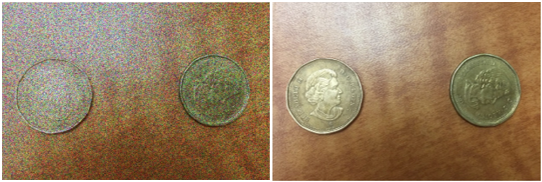
\includegraphics[width=0.7\linewidth]{Figures/specklefilter2}
		\caption{On the left is an image put through a speckle filter in Matlab. On the right is the original image.}
		\label{fig:specklefilter2}
	\end{figure}
	A problem with using an OCT interferometer is that ‘speckle’ noise exists, which ultimately reduces the quality of the image. Speckle is a phenomenon that is caused by interference of the reflected wave at the photo-detector. Speckle noise is evident when trying to image non-fluid structures (such as hard tissue). As the wave propagates it becomes distorted due to “low-angle multiple forward scattering and diffuse multiple backscattering of coherent photons”. \cite{Popescu2007}

	In OCT interferometry imaging, photons are detected after one backscattering event for most relevant information, but when a wave is propagated through a dense biological sample it experiences numerous scattering events (in OCT interferometry). These scattering events increase the likelihood for photons to change their travel distance comparative to their airborne path which results in speckle noise reducing the image quality. \cite{Popescu2007}

	To display the effects of speckling on an image refer to Figure \ref{fig:specklefilter2}. Using $imnoise(I,'speckle',v)$ in Matlab to create a filter that would add multiplicative noise to an image. As seen on the left the image resolution is decreased significantly after adding speckling noise especially in the area of high light reflectivity off of the table.

	\subsection{\label{sec:level2} Possible Solutions for Speckle Noise}
	As technology progress in imaging processing, techniques are being developed to help reduces the effects of speckle noise when using OCT. Some of these methods include decreasing spatial and temporal coherence of the laser used. While more trivial techniques such as phase-domain processing and zero-adjustments are used to improve image quality due to speckle noise. \cite{Popescu2007}

	\section{\label{sec:level1} OCT Image Aquisition and Preparation}

	\subsection{\label{sec:level2} Aquiring and Visualizing OCT Images}
	While many published reports contain printed images of OCT captures, getting raw data was necessary to make realistic observations on the effects of using digital filtering. 3D OCT captures of healthy individuals were obtained from a publised proceeding comparing OCT scans of healthy individuals \cite{tahereh_2014}. The scans were provided in .mat file format. The size of each volume provided by these scans was 650 x 512 x 128 voxels. Each voxel had a resolution of 11.72 x 46.88 x 3.54 $\mu$m. We were able to view an interactive 3D volume from the provided .mat files using a script published on MathWorks file exchange titled '3D Volume Visualization' \cite{stough}. A capture of the visualizan can be seen in figure \ref{fig:3dvol}.

	\subsection{\label{sec:level2} Slicing and Preparing a 2D Image for Processing}
	Upon importing the .mat files into Matlab, they took the form of a 650 x 512 x 128 double data type. The following Matlab code shows the process of taking the middle XY slice and creating a greyscale image.
	\begin{figure}
		\centering
		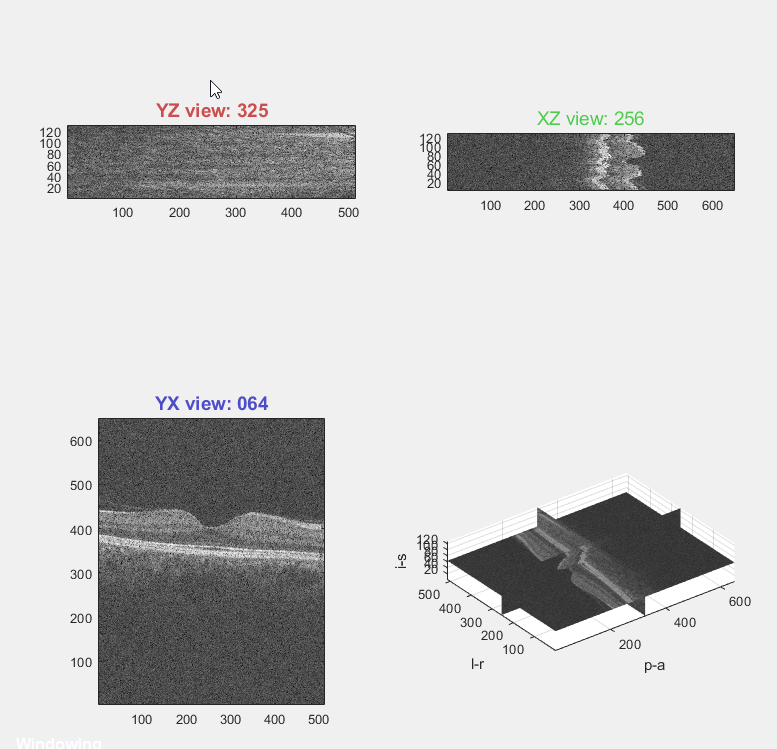
\includegraphics[width=0.7\linewidth]{Figures/3dvol}
		\caption{3D Volume Visualization Capture}
		\label{fig:3dvol}
	\end{figure}

	\section{\label{sec:level1} Scope of DSP Methods Used}
	This report will focus on 2D image filtering methods which can be applied using Matlab. To apply the supplied image filters to these images the following code was used to take a slice of an image in the XY plane.

	$$\text{(Talk more about types of methods used.)}$$
	\subsection{\label{sec:level2} Wiener Filter}
	The 2D Wiener filter is a processing technique which is capable of not only improving resolution but as well signal-to-noise (SNR) ratio of particular image. This low-pass filter is an optimal trade-off between inverse filtering and noise smoothing. This filter is also referred to as a local linear minimum mean square error which means [LLMMSE] it is the optimal estimator in the sense of mean squared error (MSE). Where LLMMSE and MSE is determined by:
$$
\begin{bmatrix}
R_{xx}[0] & R_{xx}[-1] & ... & R_{xx}[1-N]\\
R_{xx}[1] & R_{xx}[0] & ... & R_{xx}[2-N]\\
\vdots & \vdots & \ddots & \vdots \\
R_{xx}[N-1] & R_{xx}[N-2] & ... & R_{xx}[0]
\end{bmatrix}
\begin{bmatrix}
h[0]\\
h[1]\\
\vdots\\
h[N-1]
\end{bmatrix}
$$
$$
=
\begin{bmatrix}
R_{yx}[0]\\
R_{yx}[1]\\
\vdots\\
R_{yx}[N-1]
\end{bmatrix}
$$

$$R_{ee}[m]=R_{yy}[m]-R_{yy}[m] = R_{yy}[m]-h[m] \times R_{xy}[m]$$

Where $R_{xx}$ is the received signal, N is the length, then there are N equations in the N unrestricted values of h[n] and h[m] is the impulse response of the filter \cite{Oppenheim_2015}.


\subsection{\label{sec:level2} Enhanced Lee Filter}
The Lee filter applies a spatial filter to each pixel which filters data based on local statistics calculated within a square window. The value of the center pixel is replaced by a value calculated using the neighbouring pixels. Implements similar characteristics of the Wiener filter in the sense it uses MSE but also has edge preserving features \cite{leefilter}. The pixels are classified into:
\\
Homogenous: where the pixel value is replaced by an average of the filter window
\\
Heterogenous: where the pixel value is replaced by a weighted average
\\
Point: where the pixel value is unchanged.
\\
\\
The resultant gray value R for the pixels is then represented as:

$$R = I_{m} for C_{i} \leq C_{u}$$
$$R = I_{m} \times W+I_{c} \times (1-W) \text{ for } C_{u}<C_{i}<C_{max}$$
$$R = I_{c} for C_{i} \geq C_{max}$$

Where:
\\
	$I_{m}$ = mean value of intensity within the kernel
	\\
	$I_{c}$ = center pixel in the kernel
	\\
	$C_{i}$ = S/$I_{m}$
	\\
	$C_{u}$ = $\sqrt{1/(number of locks)}$
	\\
	W				= $\exp{-\zeta(C_{i}-C_{u})/(C_{max}-C_{i})}$
	\\
	S       = standard deviation of intensity within the kernel
	\cite{radarlee}




	\section{\label{sec:level1} Conclusion}





	\bibliographystyle{apa}
	\bibliography{apssamp}% Produces the bibliography via BibTeX.

\end{document}
%
% ****** End of file apssamp.tex ******
